\documentclass[aspectratio=169]{beamer}
\usepackage[square,numbers]{natbib}
\bibliographystyle{apalike}
\title[Stibo Systems Case Presentation]{UX Architecture for Data Collaboration}
\date[]{\today}
\author[]{Henrik Korsgaard}
\institute{DEPARTMENT OF COMPUTER SCIENCE} % Type in A
\usetheme{henrikkorsgaard}

\usepackage{multicol}

\usetikzlibrary{shapes.geometric, shapes.symbols}
\usepackage{tikzpeople}
\usetikzlibrary{arrows.meta}
\usepackage{fontawesome5}
\usepackage{changepage}

\makeatletter
\newbox\@backgroundblock
\newenvironment{backgroundblock}[2]{%
  \global\setbox\@backgroundblock=\vbox\bgroup%
    \unvbox\@backgroundblock%
    \vbox to0pt\bgroup\vskip#2\hbox to0pt\bgroup\hskip#1\relax%
}{\egroup\egroup\egroup}
\addtobeamertemplate{background}{\box\@backgroundblock}{}
\makeatother

\makeatletter
    \newsavebox\restorebox
\newenvironment{restoretext}%
    {\@parboxrestore% 
     \begin{adjustwidth}{-8mm}{-8mm}%
                \begin{lrbox}{\restorebox}%
                \begin{minipage}{\linewidth}%
    }{\end{minipage}\end{lrbox}
        \usebox\restorebox
        \end{adjustwidth}
     }
\makeatother

\begin{document}

\begin{frame}
\maketitle
\end{frame}

\begin{frame}{Outline}
    \begin{columns}
        \begin{column}{0.5\textwidth}
            \begin{itemize}
                \item UX research process
                \item Results and observations
                \item Information architecture
                \item Interaction design
            \end{itemize}
        \end{column}
        \begin{column}{0.5\textwidth}
            As a newly hired UX architect, your initial task is to create an outline for the UX work in a project aimed at improving the UX of the \textbf{collaboration tooling} in an existing online Excel-like table system.\\
            \vspace{1em}
            {\color{HenrikFontLight}\dots assume that you have the necessary budget for it.}
        \end{column}
    \end{columns}
\end{frame}

\begin{frame}{UX Research - key questions}
    \vspace{1em}
    \begin{columns}
        \begin{column}{0.6\textwidth}
            \textbf{Why, how, and when do users collaborate?}\\
            \vspace{1em}
            \begin{itemize}
                \small
                \item What are the primary tasks and objectives?
                \item What are the different roles and responsibilities in collaboration? 
                \item How do remote work impact the user experience?
                \item What other tools do they use to support the tasks -- planning, communication, analysis etc.?
            \end{itemize}
        \end{column}
        \begin{column}{0.4\textwidth}
            \begin{figure}[h]
                \centering
                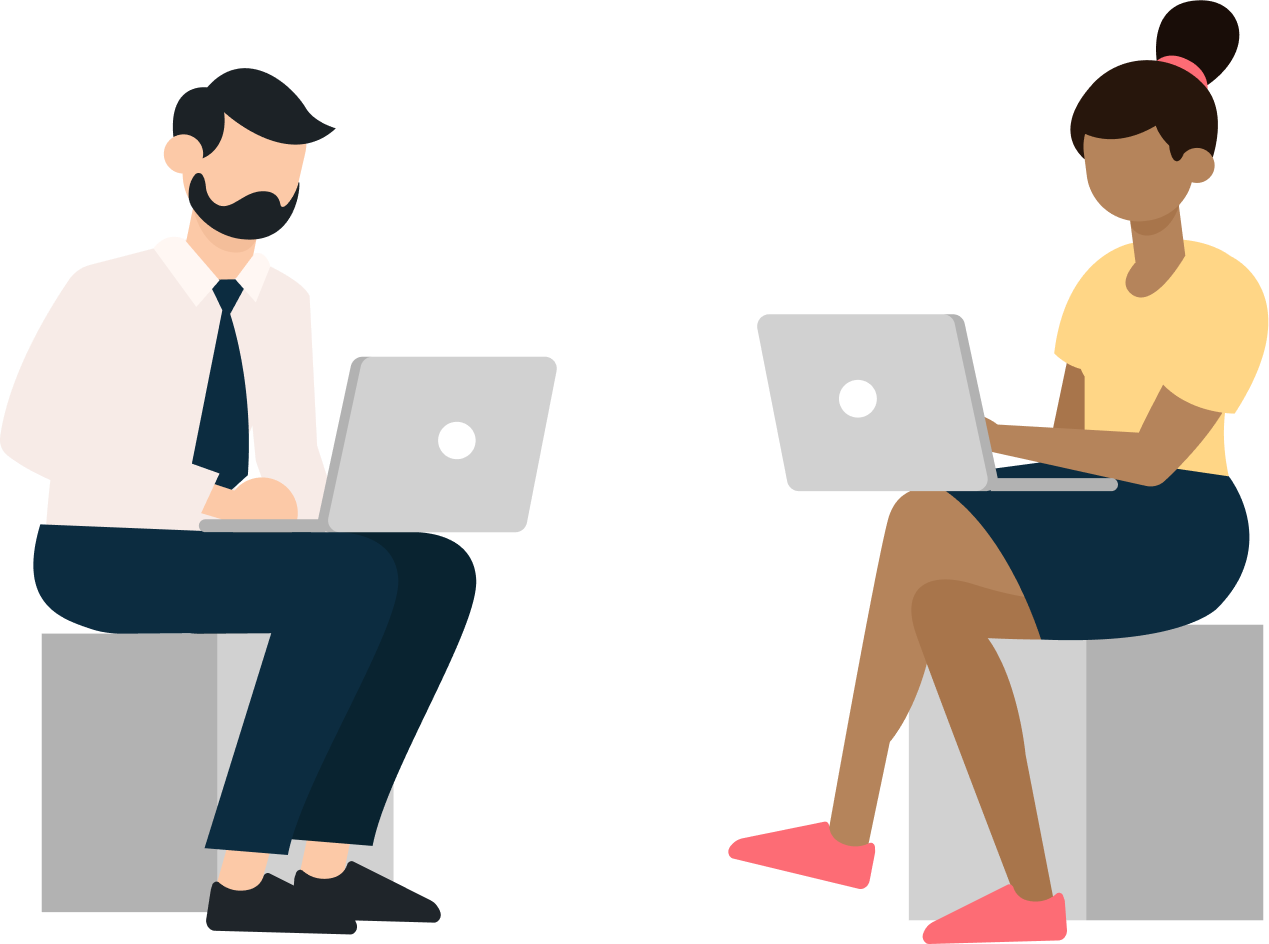
\includegraphics[width=0.8\textwidth]{images/collaborators.png}
            \end{figure}
        \end{column}
    \end{columns}
    \let\thefootnote\relax\footnotetext{Ida Larsen-Ledet, and Henrik Korsgaard. Territorial functioning in \textbf{collaborative writing}. CSCW 2019\\Ida Larsen-Ledet, Henrik Korsgaard, and Susanne Bødker. \textbf{Collaborative writing} across multiple artifact ecologies.CHI 2020}
\end{frame}


\begin{frame}{UX Research}
    \vspace{-1em}
    \begin{columns}[t]
        \begin{column}{0.5\textwidth}
            \small
            \textbf{Discover}
            \begin{enumerate}
                \item Contextual interviews of collaborative session(s)
                \item Task flow analysis
                \item Internal/external research
                \item Workshops (?)
                \item Analytics (?)
            \end{enumerate}
        \end{column}
        \begin{column}{0.5\textwidth}
            \small
            \textbf{Define}
            \begin{itemize}
                \item Collaborative task objectives 
                \item Scenarios, personas and user journeys
                \item Information concepts and architecture
                \item UX quality criteria and KPIs
            \end{itemize}
        \end{column}
    \end{columns}
    \begin{restoretext}
    \begin{backgroundblock}{7mm}{50mm}
    \centering
    \resizebox{1\textwidth}{!}{%
    \begin{tikzpicture}

        \node[diamond,fill=HenrikDark!3, minimum width = 4.5cm, minimum height = 4.5cm] (d) at (1.1,1) {};
        \node[diamond,fill=HenrikDark!3, minimum width = 4.5cm, minimum height = 4.5cm] (d) at (5.5,1) {};

        \node[signal to=east, signal from=west,shape=signal, draw, minimum width = 2.15cm, minimum height = 0.5cm,white, fill=HenrikDark] at (0.1,1) {\tiny Discover};
        \node[signal to=east, signal from=west, shape=signal, draw, minimum width = 2.3cm, minimum height = 0.5cm,white,fill=HenrikDark] at (2.2,1) {\tiny Define};
        \node[signal to=east, signal from=west, shape=signal, draw, minimum width = 2.3cm, minimum height = 0.5cm] at (4.37,1) {\tiny Prototype};
        \node[signal to=east, signal from=west, shape=signal, draw, minimum width = 2.3cm, minimum height = 0.5cm, fill=white] at (6.54,1) {\tiny Evaluate};
        \node[signal to=east, signal from=west, shape=signal, draw, minimum width = 2.3cm, minimum height = 0.5cm, fill=white] at (8.7,1) {\tiny Integrate}; 
    \end{tikzpicture}
    }
\end{backgroundblock}
\end{restoretext}
\end{frame}

\begin{frame}{UX Research -- iterate where needed}
    \vspace{-1em}
    \begin{columns}[t]
        \begin{column}{0.5\textwidth}
            \small
            \textbf{Prototype}
            \begin{itemize}
                \item Collaborative user flow
                \item Information architecture and UI design
                \item Key UI components and technical features
            \end{itemize}
        \end{column}
        \begin{column}{0.5\textwidth}
            \small
            \textbf{Evaluate}
            \begin{itemize}
                \item Internal review and testing
                \item User feedback (informal/think aloud)
                \item Review UX quality criteria and KPIs
            \end{itemize}
        \end{column}
    \end{columns}
    \begin{restoretext}
    \begin{backgroundblock}{7mm}{50mm}
    \centering
    \resizebox{1\textwidth}{!}{%
    \begin{tikzpicture}

        \node[diamond,fill=HenrikDark!3, minimum width = 4.5cm, minimum height = 4.5cm] (d) at (1.1,1) {};
        \node[diamond,fill=HenrikDark!3, minimum width = 4.5cm, minimum height = 4.5cm] (d) at (5.5,1) {};

        \node[signal to=east, signal from=west,shape=signal, draw, minimum width = 2.15cm, minimum height = 0.5cm] at (0.1,1) {\tiny Discover};
        \node[signal to=east, signal from=west, shape=signal, draw, minimum width = 2.3cm, minimum height = 0.5cm] at (2.2,1) {\tiny Define};
        \node[signal to=east, signal from=west, shape=signal, draw, minimum width = 2.3cm, minimum height = 0.5cm, white, fill=HenrikDark] at (4.37,1) {\tiny Prototype};
        \node[signal to=east, signal from=west, shape=signal, draw, minimum width = 2.3cm, minimum height = 0.5cm, white, fill=HenrikDark] at (6.54,1) {\tiny Evaluate};
        \node[signal to=east, signal from=west, shape=signal, draw, minimum width = 2.3cm, minimum height = 0.5cm, fill=white] at (8.7,1) {\tiny Integrate}; 
    \end{tikzpicture}
    }
\end{backgroundblock}
\end{restoretext}
\end{frame}

\begin{frame}{Collaborative scenarios}
    \setlength{\leftmargini}{0.5cm}
    \begin{columns}[t]
        \begin{column}{0.33\textwidth}
            \textbf{\small 1. Collaborative projects}
            \begin{itemize}
                \scriptsize
                \item Peers collaborate on a larger project
                \item Different responsibilities and expertise
                \item Mixed focus collaboration with a high degree of coordination
                \item Multiple data views
            \end{itemize}
        \end{column}
        \begin{column}{0.33\textwidth}
            \textbf{\small 2. Real-time collaboration}
            \begin{itemize}
                \scriptsize
                \item Peers collaborate on smaller (urgent) tasks
                \item Real-time collaboration
                \item Shared task focus 
                \item Few data views
            \end{itemize}
        \end{column}
        \begin{column}{0.33\textwidth}
            \textbf{\small 3. Training}
            \begin{itemize}
                \scriptsize
                \item Expert user provide training and onboarding of novices
                \item Focused on learning the application and/or data
                \item Tailored data views and exercises
            \end{itemize}
        \end{column}
    \end{columns}
\end{frame}

\begin{frame}{Key UX qualities}
    \begin{columns}
        \begin{column}{0.7\textwidth}
            \small
            \begin{itemize}
                \item Collaboration should be responsive and clearly communicated
                \item Sharing with collaborators should include task assignment and notes
                \item Important to know who did what in a shared view (awareness, track changes, accountability etc.)
                \item Support sandbox experimentation and analysis before publishing
                \item Collaborative features should not compromise existing task/productivity features
            \end{itemize}
        \end{column}
        \begin{column}{0.4\textwidth}
            \vspace{-2em}
            \begin{figure}[h]
                \centering
                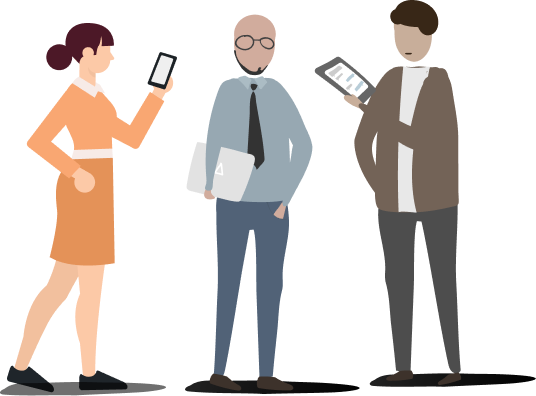
\includegraphics[width=1\textwidth]{images/Users.png}
            \end{figure}
        \end{column}
    \end{columns}
\end{frame}

\begin{frame}{Information Design: Data views as first class objects}
    \begin{columns}
        \begin{column}{0.4\textwidth}
            \begin{itemize}
                \footnotesize
                \item Main information artifact when collaborating -- it's what we share and work on
                \item A data view encapsulate a data source, users, and the revision history
                \item Views can be published in formats fitting the consumer needs
            \end{itemize}
        \end{column}
        \begin{column}{0.6\textwidth}
            \begin{figure}[h]
                \centering
                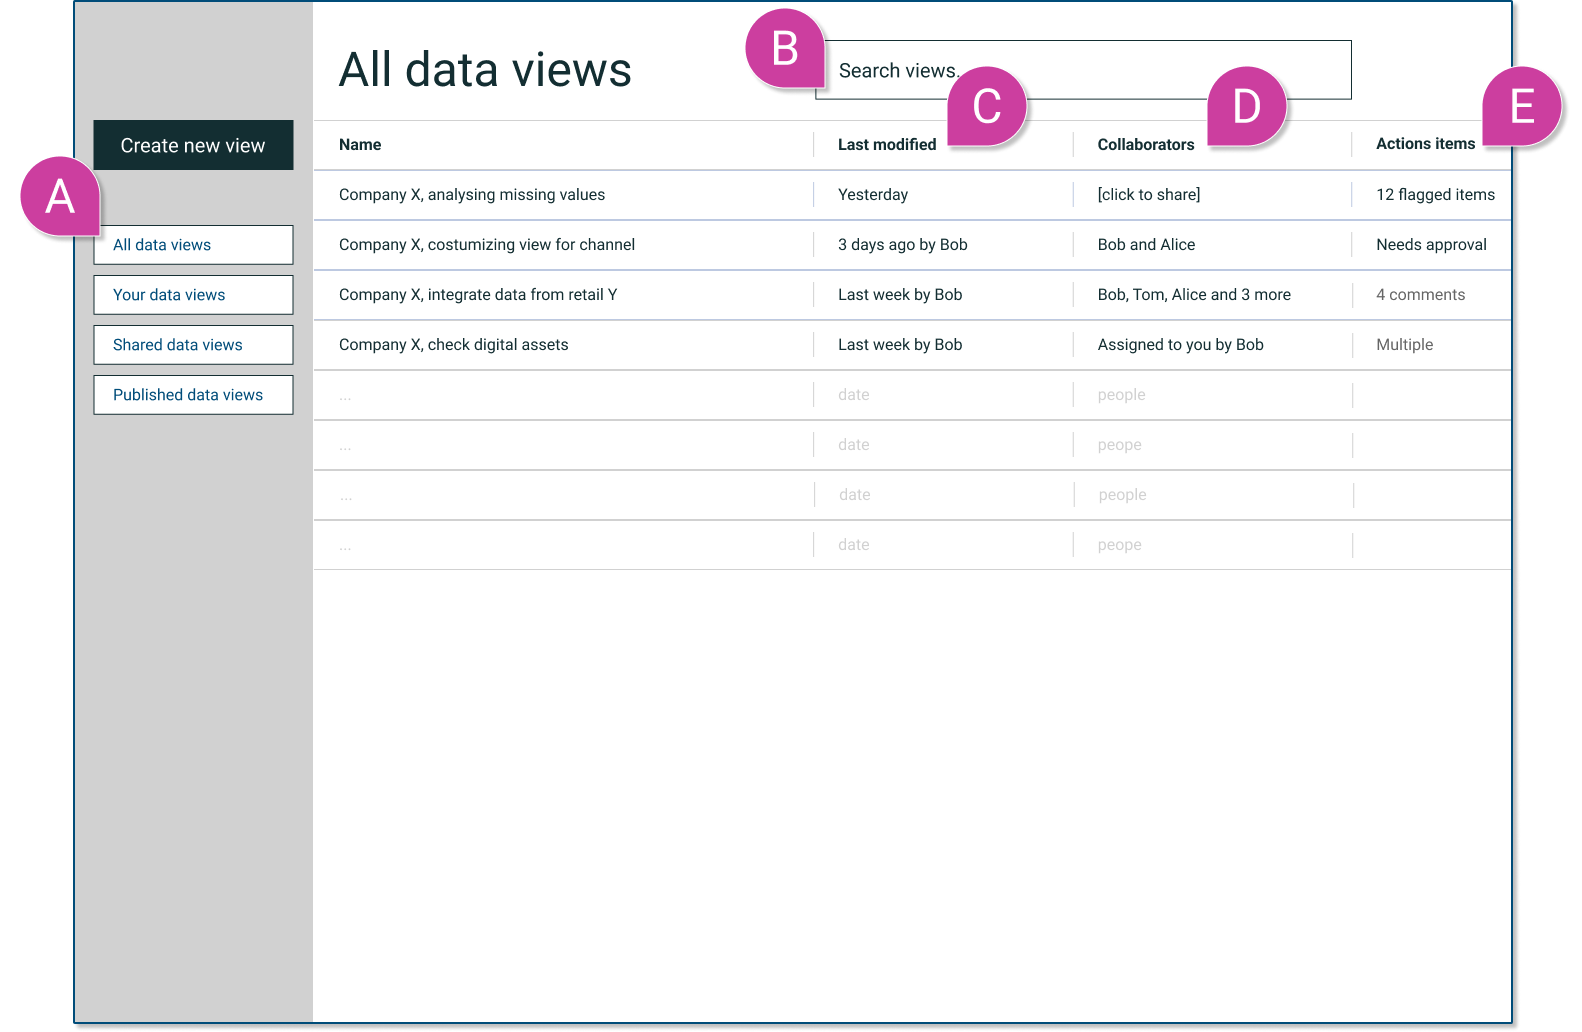
\includegraphics[width=1.1\textwidth]{images/all-views-with-marks.png}
            \end{figure}
        \end{column}
    \end{columns}
\end{frame}

\begin{frame}{Creating and sharing a\\ data view}
    \begin{figure}[h]
        \centering
        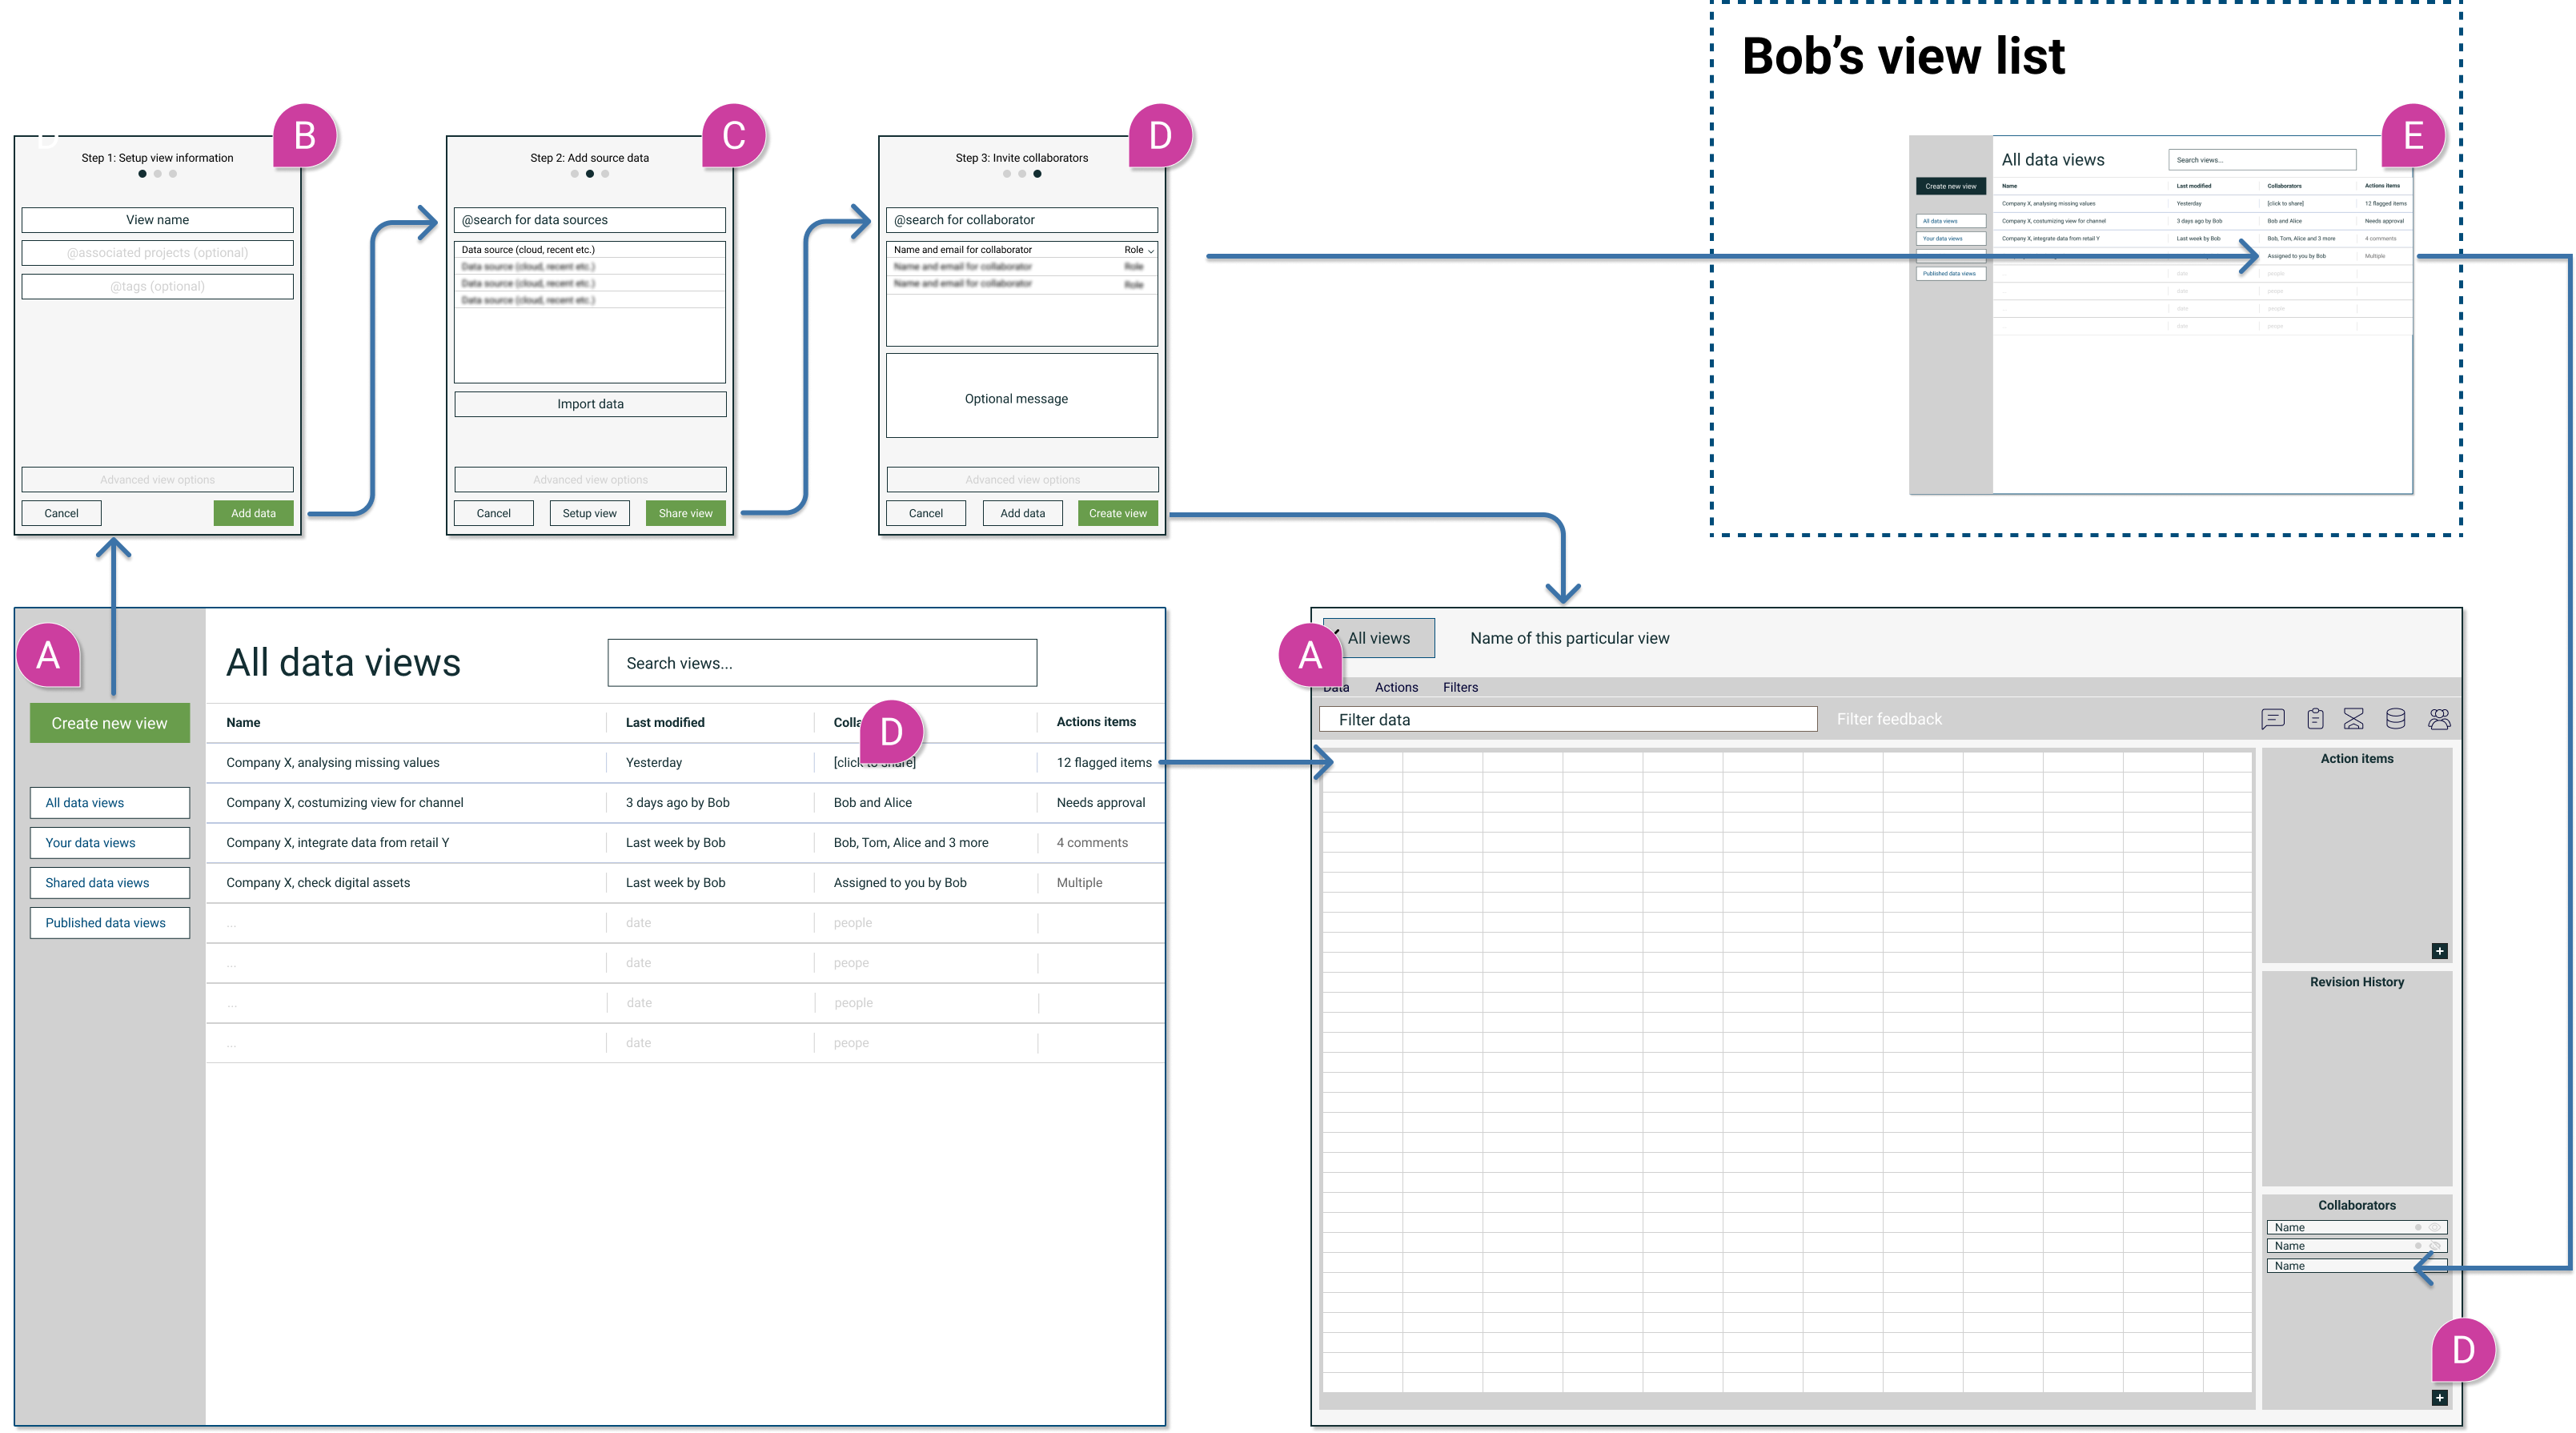
\includegraphics[width=1\textwidth]{images/create-new-view-flow.png}
    \end{figure}
\end{frame}

\begin{frame}{Collaborative tooling with tabular data}
    \begin{columns}
        \begin{column}{0.4\textwidth}
            \begin{itemize}
                \small
                \item \textbf{Action items} supports different roles and tasks
                \item \textbf{Revision history} supports shared track changes and accountability
                \item \textbf{Collaborator pane} supports awareness and social navigation
            \end{itemize}
        \end{column}
        \begin{column}{0.6\textwidth}
            \begin{figure}[h]
                \centering
                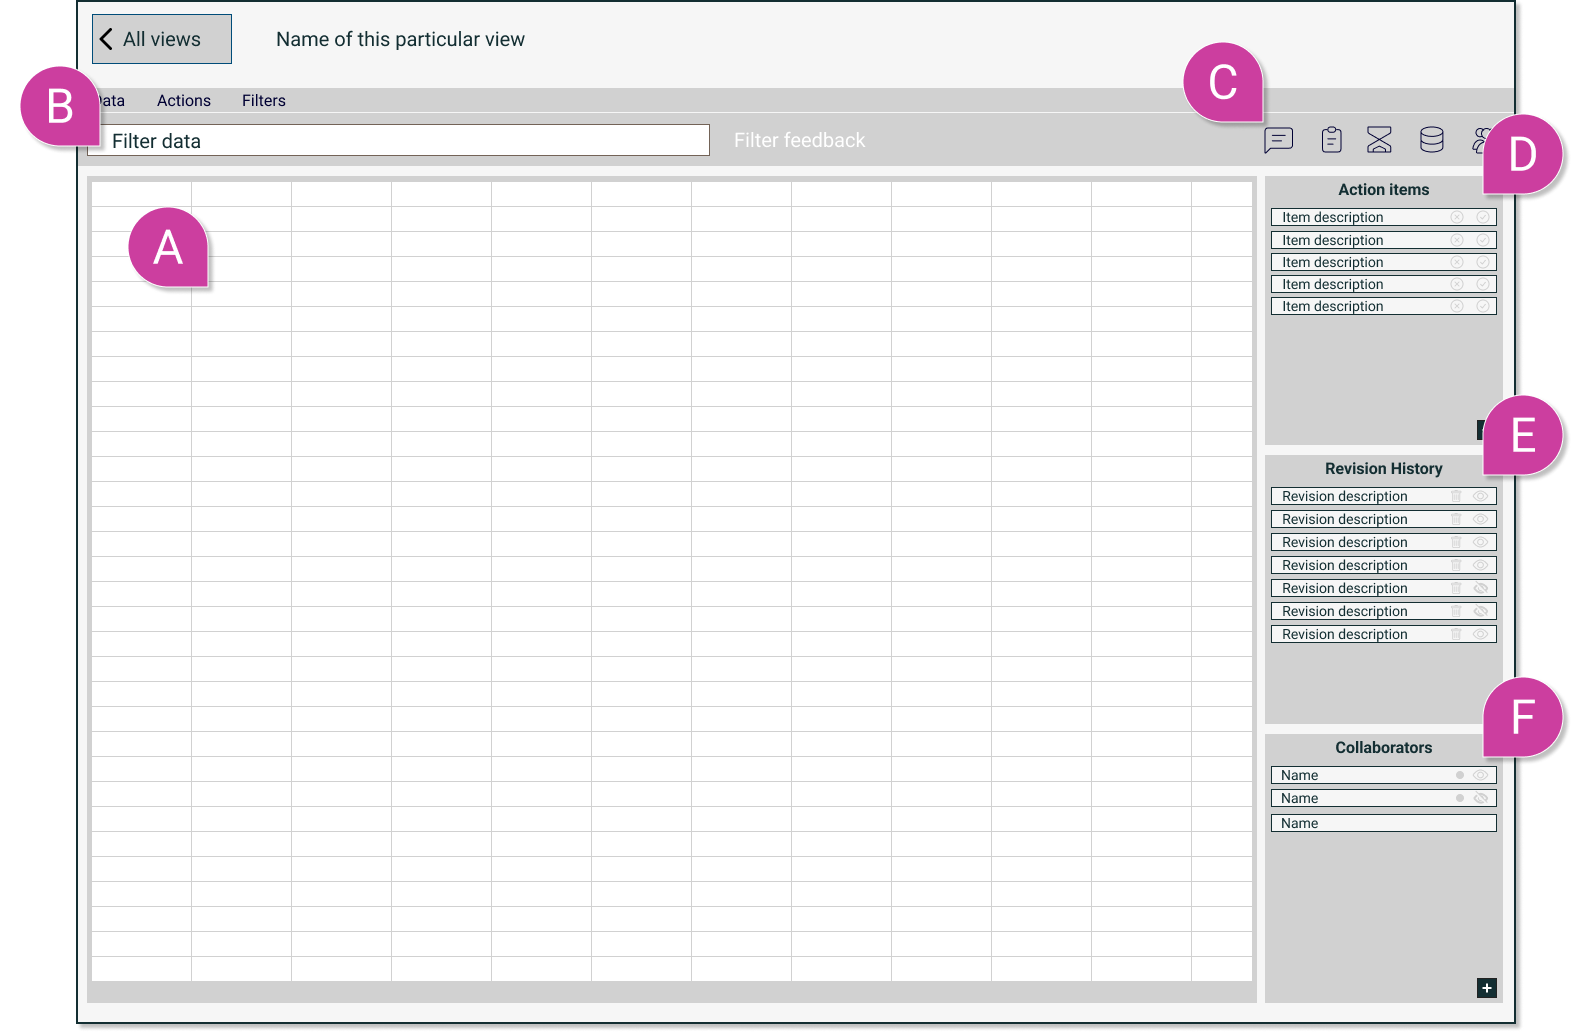
\includegraphics[width=1\textwidth]{images/filter-view-with-marks.png}
            \end{figure}
        \end{column}
    \end{columns}
\end{frame}

\begin{frame}{Assign action item to collaborators}
    \vspace{2em}
    \begin{restoretext}
    \begin{figure}[h]
        \centering
        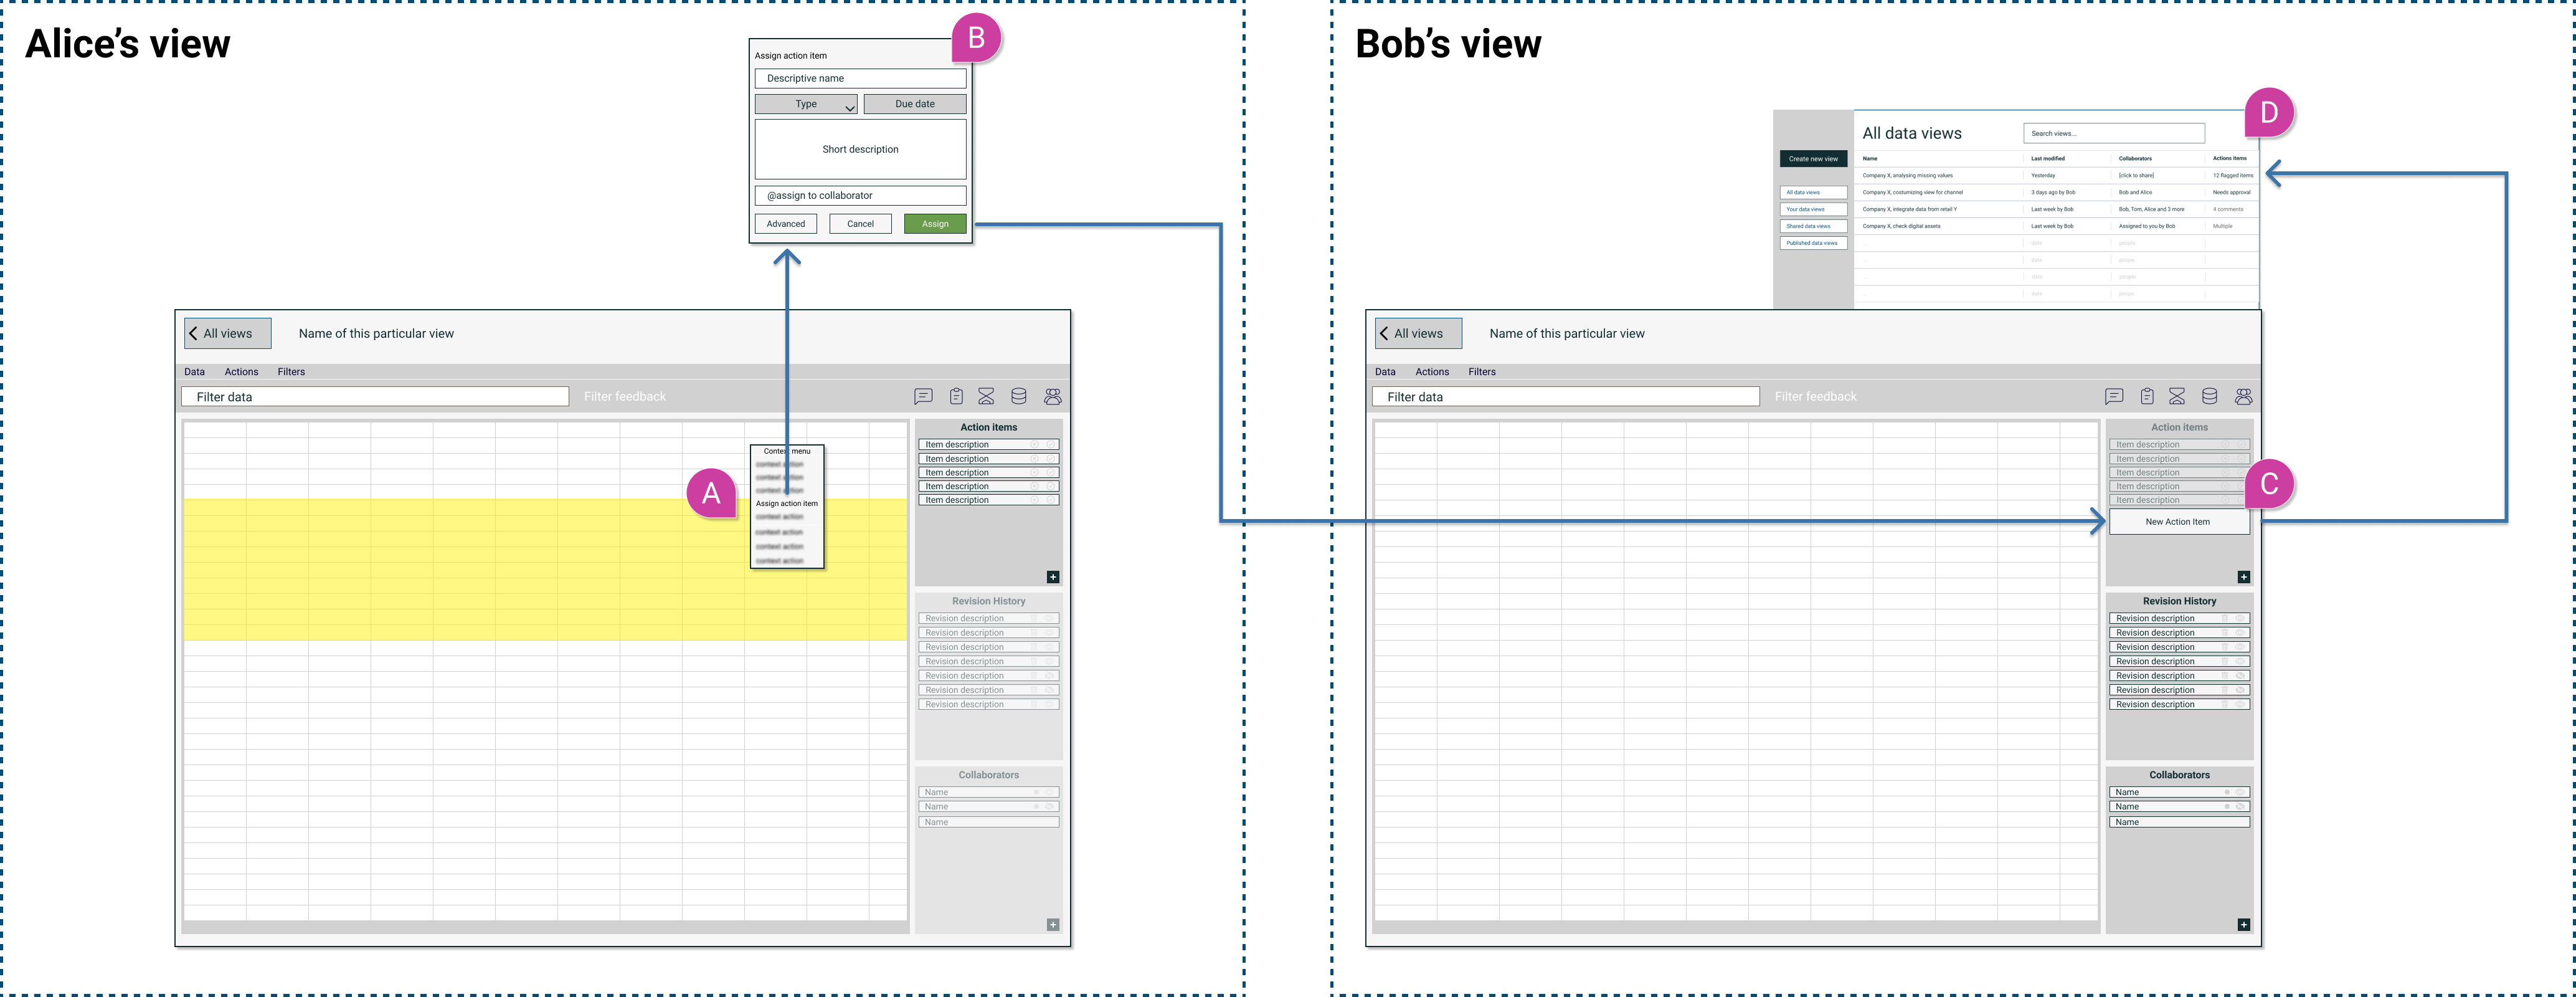
\includegraphics[width=1\textwidth]{images/assign-action-item.png}
    \end{figure}
\end{restoretext}
\end{frame}

\begin{frame}{Revision history as key\\ collaboration support}
    \begin{columns}
        \begin{column}{0.5\textwidth}
            \begin{itemize}
                \small
                \item Data operations as the replicated objects (CRDT)
                \item Support task resumption, accountability and finding stuff
                \item Support experimentation -- you can always roll back changes
                \item A set of operations can be applied to other data views (macros)
            \end{itemize}
        \end{column}
        \begin{column}{0.5\textwidth}
            \begin{figure}[h]
                \vspace{-4em}
                \centering
                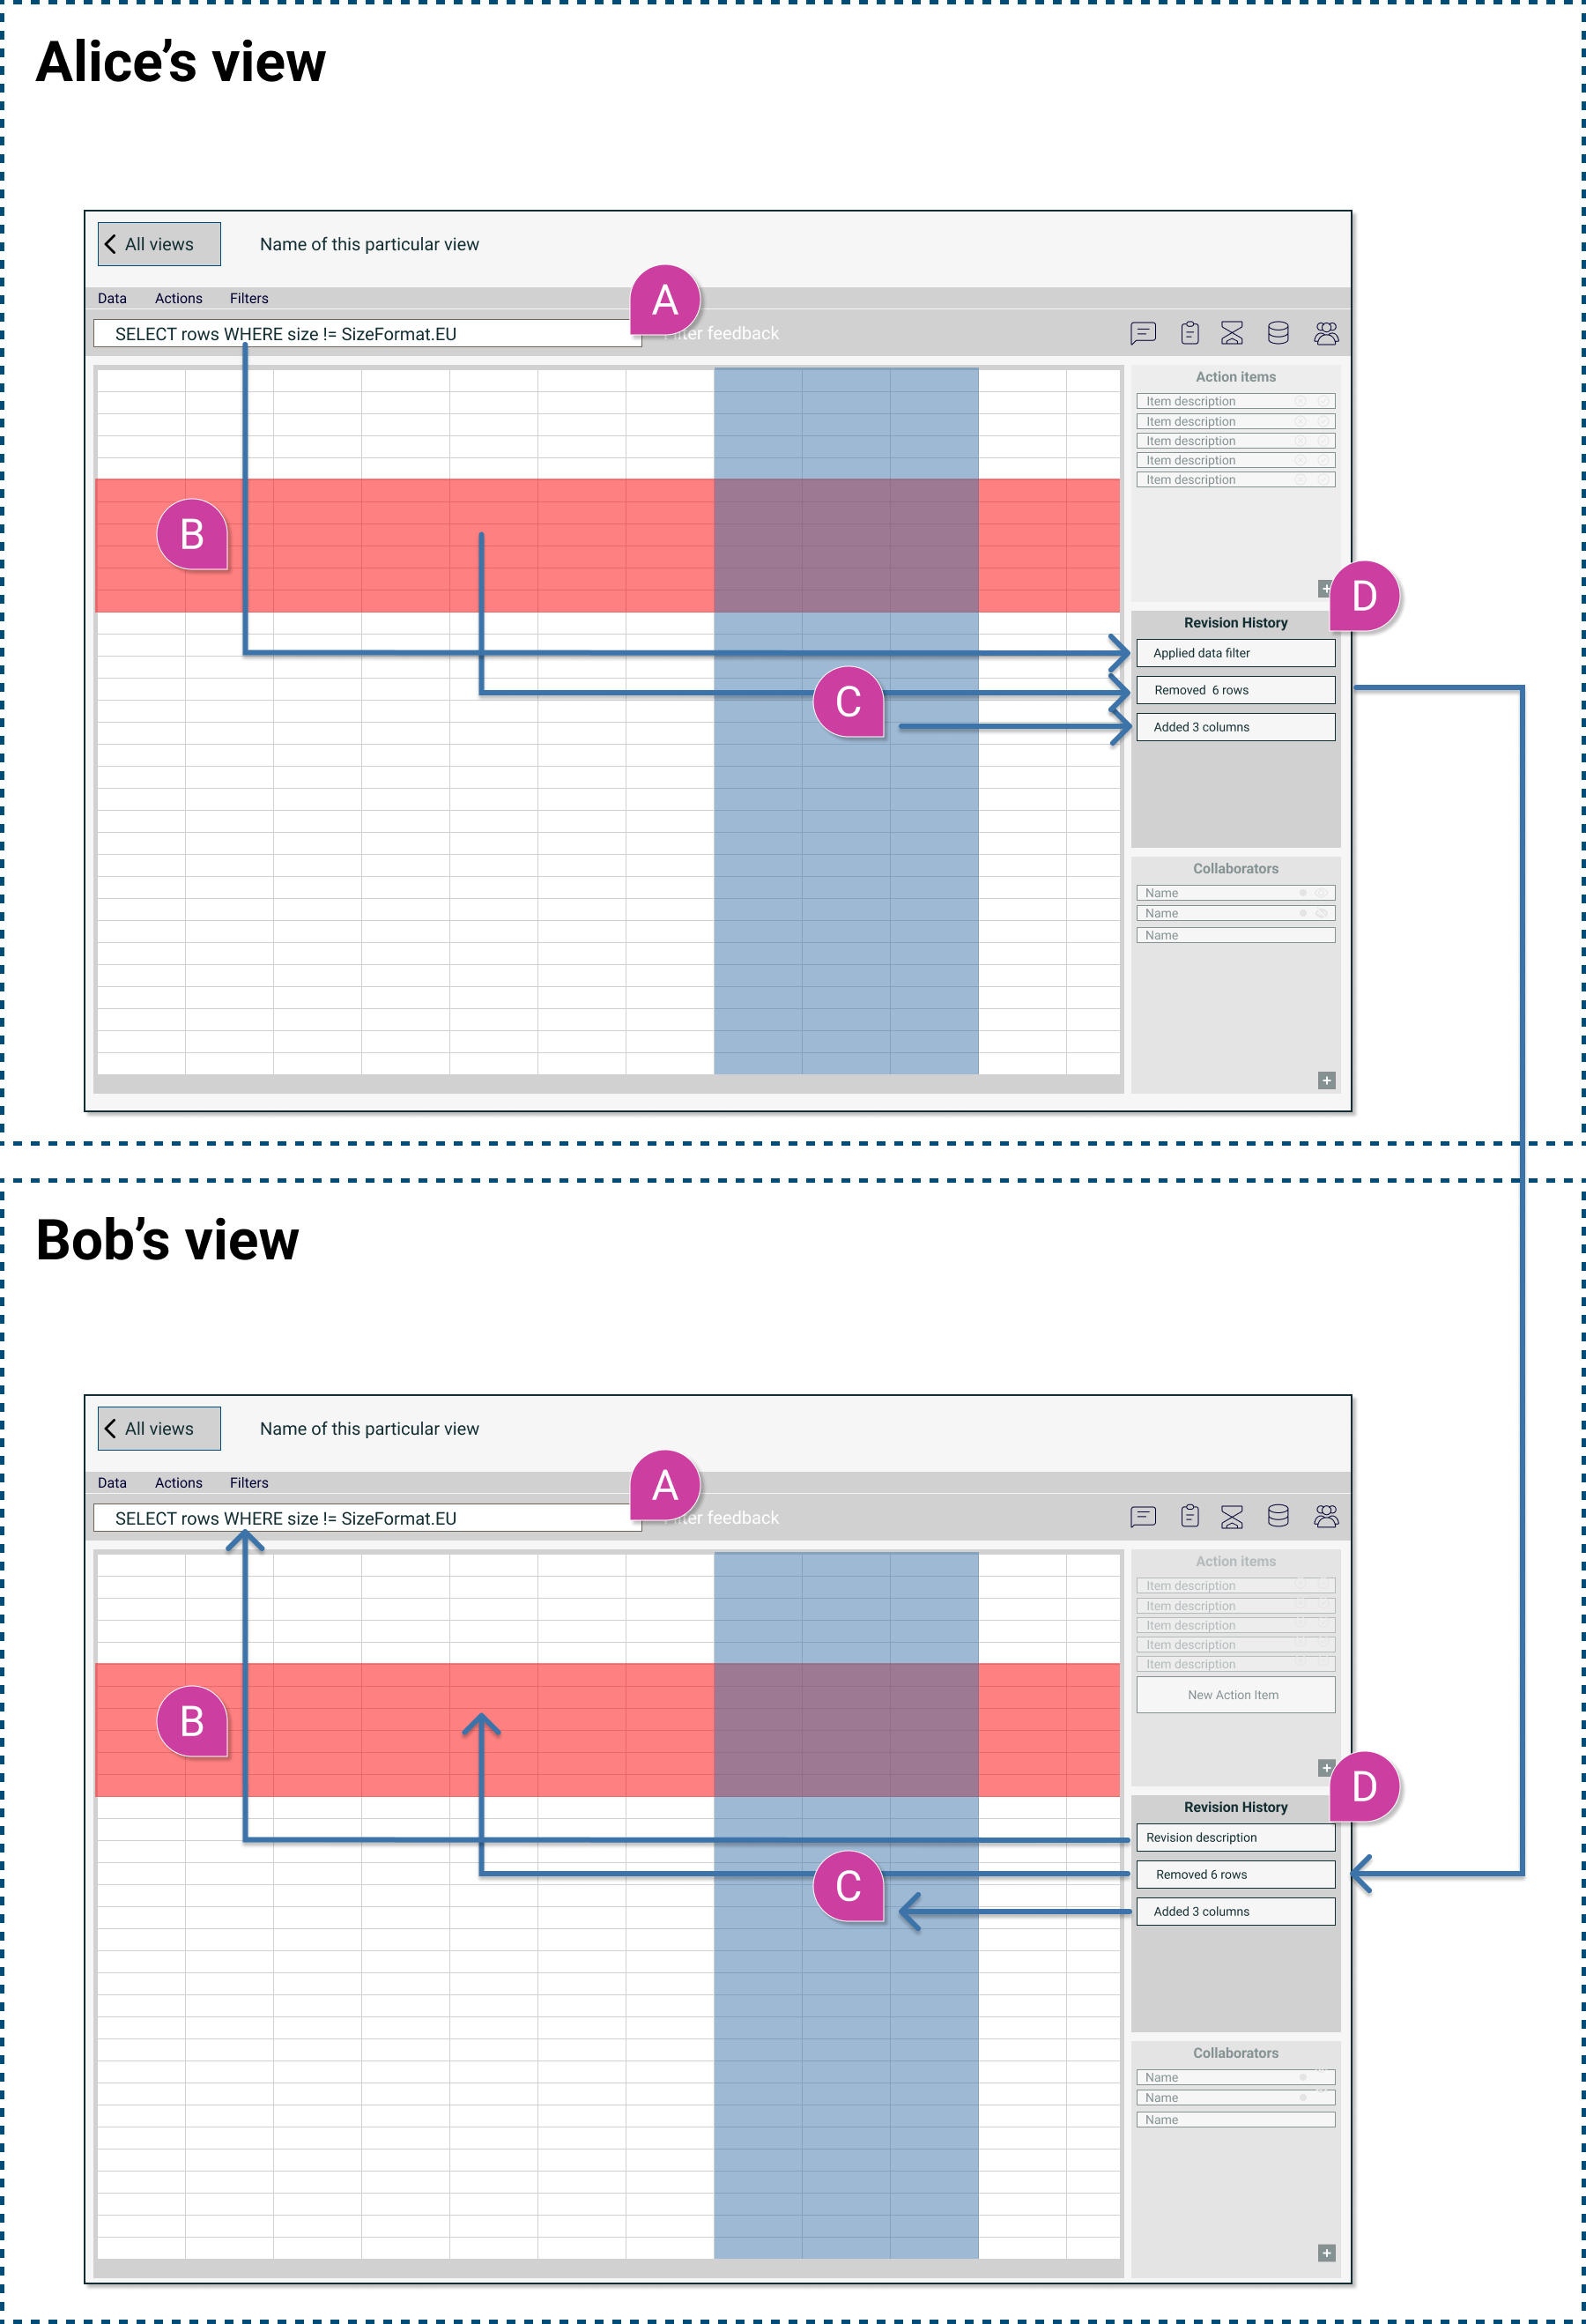
\includegraphics[width=0.9\textwidth]{images/shared-history.png}
            \end{figure}
        \end{column}
    \end{columns}
\end{frame}

\begin{frame}[DarkSlide]{}
    \vspace{3em}
    \centering
    \Large THANK YOU\\
\end{frame}

\end{document}